\chapter{薛宝钗小恙梨香院\quad 贾宝玉大醉绛芸轩}
\qi{幻情浓处故多嗔,岂独颦儿爱妒人。
莫把心思劳展转,百年事业总非真。
}\par
题曰:\par
古鼎新烹凤髓香,
\zhu{
凤髓:极言香的原料之珍异。
类似地,第五回的“麟髓之醅”、“凤乳之麯”均极言酿造仙酒的原料之珍异。
}
那堪翠斝贮琼浆。
\zhu{
斝:音“甲”,古代酒器,圆口平底。
}\par
莫言绮縠无风韵,
\zhu{縠:音“胡”,有皱纹的纱。
绮縠:犹言绮罗,指代女子,这里指宝钗。
}
试看金娃对玉郎。
\zhu{金娃:指宝钗。玉郎:指宝玉。}
\par
话说凤姐和宝玉回家,见过众人。
宝玉先便回明贾母,秦钟要上家塾之事,自己也有了个伴读的朋友,正好发奋,\jia{未必。
\ping{毒舌。
}}又着实的称赞秦钟的人品行事,最使人怜爱。
\meng{“怜爱”二字写出宝玉真神,若是别个断不肯透露。
凤姐帮话是为秦氏,用意屈尽人情。
\zhu{屈尽:穷尽。}
}凤姐又在一旁帮着说“过日他还来拜老祖宗”等语,说的贾母喜悦起来。
\jia{止此便十成了,不必繁文再表,故妙。
偷渡金针法。
\zhu{
偷渡金针:同“偷度金针”、“金针暗度”。
度:授与,传授。比喻把高超的技艺偷偷传授给别人。
唐·冯翊子《桂苑丛谈·史遗》:“(采娘)七夕夜陈香筵祈于织女。是夕梦云舆羽盖蔽空,驻车命采娘曰:‘吾织女,祈何福?’曰:‘愿丐巧耳。’乃遗一金针,长寸余,缀于纸上,置裙带中,令三日勿语,汝当奇巧。”
后也以刺绣譬喻作诗文者别有巧妙,明清小说、戏剧评点家也常用来评点小说、戏剧中的巧妙章法和构思。
从《红楼梦》有关回的正文看,作批者是指曹雪芹表面在写一回事,而实际有更深的、另外的含义,或者是运用巧妙的艺术手法而不露痕迹。
}
}凤姐又趁势请贾母后日过去看戏。
贾母虽年高,却极有兴头。
\jia{为贾母写传。
}至后日,又有尤氏来请,遂携了王夫人、林黛玉、宝玉等过去看戏。
至晌午,贾母便回来歇息了。
\jia{叙事有法,若只管写看戏,便是一无见世面之暴发贫婆矣。
写“随便”二字,兴高则往,兴败则回,方是世代封君正传。
且“高兴”二字,又可生出多少文章来。
}\ping{贾母也可能虽有兴头,但还是年老体弱,支撑不住。
第七十六回中秋聚会之时,贾母听着尤氏讲笑话,自己却“已朦胧双眼,似有睡去之态。
”贾母实则尽力支撑和家人同乐。
}王夫人本是好清净的,\jia{偏与邢夫人相犯,然却是各有各传。
}见贾母回来,也就回来了。
然后凤姐坐了首席,尽欢至晚无话。
\jia{细甚,交代毕。
}\par
却说宝玉因送贾母回来,待贾母歇了中觉,意欲还去看戏取乐,又恐扰的秦氏等人不便,\jia{全是体贴功夫。
}因想起近日薛宝钗在家养病,未去亲候,意欲去望他一望。
若从上房后角门过去,又恐遇见别事缠绕,再或可巧遇见他父亲,\jia{本意正传,实是曩时苦恼,
\zhu{曩:音“攮”,从前;过去。}
叹叹!}更为不妥,\jia{细甚。
}宁可绕远路罢了。
当下众嬷嬷丫鬟伺候他换衣服,见他不换,仍出二门去了。
众嬷嬷丫鬟只得跟随出来,还只当他去那府中看戏。
谁知到了穿堂,便向东向北绕厅后而去。
偏顶头遇见了门下清客相公詹光\jia{妙!盖沾光之意。
}\zhu{清客相公:清客:旧时依附于官僚富贵人家帮闲凑趣的门客。
相公:这里是对读书人的一般称呼,近似“先生”。
}、单聘仁\jia{更妙!盖善于骗人之意。
}二人走来,一见了宝玉,便都笑着赶上来,一个抱住腰,一个携着手,都道:“我的菩萨哥儿,\jia{没理没伦,口气毕肖。
}我说作了好梦呢,好容易得遇见了你。
”说着,请了安,又问好,唠叨了半日,方才走开。
\jia{一路用淡三色烘染、行云流水之法,写出贵公子家常不即不离气致。
\zhu{不即不离:比喻对人的态度,既不亲近,也不疏远。}
经历过者则喜其写真,未经者恐不免嫌繁。
}老嬷嬷叫住,因问:“你二位爷是从老爷跟前来的不是?”\jia{为玉兄一人,却人人俱有心事,细致。
}他二人点头道:“老爷在梦坡斋\jia{使人起遐思。
}\jia{妙!梦遇坡仙之处也。
\zhu{坡仙:苏轼,号东坡居士,后人敬称之为坡仙。}
}小书房里歇中觉呢,不妨事的。
”\jia{玉兄知己。
一笑。
}一面说,一面走了。
说的宝玉也笑了。
\par
于是转弯向北奔梨香院来。
\meng{吃冷香丸,往梨香院。
有趣。
}可巧银库房的总领名唤吴新登\jia{妙!盖云无星戥也。
\zhu{戥:音“等”,一种称量金银、药品等所用的小秤,计量单位从分厘到两,构造和原理跟杆秤相同,盛物体的部分是一个小盘子。
星:秤杆上标记斤、两、钱的小点子。
}}\ping{吴新登是银库房的总领,无星戥是没有刻度的杆秤,通过谐音联系在一起,银库房称量银两使用没有刻度的杆秤,可能暗含讽刺银库房收支混乱。
}与仓上的头目名戴良,\jia{妙!盖云大量也。
\ping{言贾府仓中积储量大。}
}还有几个管事的头目,共有七个人,从帐房里出来,一见了宝玉,赶来都一齐垂手站住。
独有一个买办名唤钱华的,\jia{亦钱开花之意。
\zhu{钱开花:联系戴良的谐音“大量”,这里的意思可能是“大量钱开(始)花(出去)”,隐晦的点出贾府财务上的流弊。}
随事生情,因情得文。
}\ping{钱华,倒过来念为“花钱”,暗合他买办的身份。
}因他多日未见宝玉,忙上来打千儿请安,\zhu{打千儿:旧时满族男子向人请安,左膝前屈,右腿后弯,上身微俯,右手下垂,行半跪礼。
}宝玉忙含笑携他起来。
\ping{宝玉在姊妹丛中处处流露小孩子的天性,和丫鬟也不分等级平等相待;但是在大人世界的应酬接待时,又不得不拿出小主人的样子,装成大人的模样。
宝玉正处在从青春世界过渡到成人世界的转折,一脚还留在青春无邪,一脚已经被世俗拽进了滚滚红尘。
}众人都笑说:“前儿在一处看见二爷写的斗方,\zhu{斗方:一种一、二尺见方的单幅笺纸,置四角于上下左右四方,写字作画其中,可张挂或收藏。
}字法越发好了,多早晚赏我们几张贴贴。
”\jia{余亦受过此骗,今阅至此,赧然一笑。
\zhu{赧:音“难”三声,(因羞愧等)脸色泛红。
}此时有三十年前向余作此语之人在侧,观其形已皓首驼腰矣,乃使彼亦细听此数语,彼则潸然泣下,余亦为之败兴。
}宝玉笑道:“在那里看见了?”众人道:“好几处都有,都称赞的了不得,还和我们寻呢。
”\meng{侍奉上人者,无此等见识、无此等迎奉者,难乎免于厌弃,呜呼哀哉。
}宝玉笑道:“不值什么,你们说给我的小幺儿们就是了。
\zhu{
幺(音“妖”):幼小。
小幺儿:身边使唤的小仆人。
}
”一面说,一面前走,众人待他过去,方都各自散了。
\jia{未入梨香院,先故作若许波澜曲折。
瞧他无意中又写出宝玉写字来,固是愚弄公子闲文,然亦是暗逗宝玉历来文课事。
\ping{宝玉作为富家公子,受到众人逢迎吹捧,如不能看透世情反而自以为是,则是被愚弄而不知。}
不然,后文岂不太突?}\par
闲言少述,\jia{此处用此句最当。
}\ping{宝玉出门一趟实在麻烦。
}且说宝玉来至梨香院中,先入薛姨妈室中来,正见薛姨妈打点针黹与丫鬟们呢。
宝玉忙请了安,薛姨妈忙一把拉了他,抱入怀内,笑说:“这么冷天,我的儿,难为你想着来,快上炕来坐着罢。
”命人倒滚滚的茶来。
宝玉因问:“哥哥不在家?”薛姨妈叹道:“他是没笼头的马,天天逛不了,那里肯在家一日。
”宝玉道:“姐姐可大安了?”薛姨妈道:“可是呢,你前儿又想着打发人来瞧他。
他在里间不是,你去瞧他。
里间比这里暖和,那里坐着,我收拾收拾就进去和你说话儿。
”\meng{作者何等笔法。
“里间里”三字,
\zhu{里间里:原文没有这三个字,可能是批书人的笔误。}
恐文气不足,又贯之以“比这里和暖”,
\zhu{和暖:原文用的是“暖和”。}
其笔真是神龙云中弄影,是必当进去的神理。
}\par
宝玉听说,忙下了炕,来至里间门前,只见吊着半旧的红紬软帘。
\zhu{紬:同“绸”。
}
\jia{从门外看起,有层次。
}宝玉掀帘一迈步进去,先就看见薛宝钗坐在炕上作针线,头上挽着漆黑油光的䰖儿,
\zhu{䰖:音“钻”三声。䰖儿:也写作“纂儿”。
妇女的发髻。}
蜜合色棉袄,
\zhu{蜜合色:淡黄如蜂蜜色。}
玫瑰紫二色金银鼠比肩褂,
\zhu{
玫瑰紫:紫玫瑰花色。
二色金:全称“二色金库锦”。花纹全部用金、银两种线织出,一般以金线为主,少部分花纹用银线装饰。
银鼠:状颇类鼬,耳小毛短,其色洁白,皮可御轻寒,极贵重。
比肩:披肩,《元史·舆服志一》:服银鼠,则冠银鼠暖帽,其上并加银鼠比肩。比肩是天子冬天在内庭大型宴会时加在质孙(一种冕服)上的服饰,用银鼠皮做成,材质高档。在正装上面加比肩,既能保暖,又不失皇家尊严,非常得体。宝钗的比肩褂是穿在袄的外面的,虽然是在闺房内,但宝钗天性庄重自律,穿的也是不太随便的衣服。
}
葱黄绫棉裙,一色半新不旧,看来不觉奢华。
唇不点而红,眉不画而翠;脸若银盆,眼如水杏。
罕言寡语,人谓藏愚;\zhu{藏愚:藏智巧于愚讷的外表之中。
}安分随时,自云守拙。
\zhu{守拙:拙于应世而淡泊自守。
}\jia{这方是宝卿正传。
与前写黛玉之传一齐参看,各极其妙,各不相犯,使[其]人难其左右于毫末。
\zhu{左右:分辩或论断其高低、优劣。范仲淹《上资政晏侍郎书》:“非敢左右其说,惟公之采择。”使人难其左右于毫末:宝钗和黛玉根本无法分出高低优劣。}
}\jia{画神鬼易,画人物难。
写宝卿正是写人之笔,若与黛玉并写更难。
今作者写得一毫难处不见,且得二人真体实传,非神助而何?}宝玉一面看,一面口内问:“姐姐可大愈了?”宝钗抬头\jia{与宝玉迈步针对。
}只见宝玉进来,\jia{此则神情尽在烟飞水逝之间,一展眼便失于千里矣。
}连忙起来含笑答说:“已经大好了,倒多谢记挂着。
”说着,让他在炕沿上坐了,即命莺儿斟茶来。
一面又问老太太、姨妈安,别的姊妹们都好。
\jia{这是口中如此。
}一面\jia{“一面”二,口中眼中,神情俱到。
}看宝玉头上戴着累丝嵌宝紫金冠,\zhu{累:堆叠,重叠。
}额上勒着二龙抢珠金抹额,
\zhu{抹额:系绑在额头上的布巾。}
身上穿着秋香色立蟒白狐腋箭袖,\zhu{
秋香色:深黄色。
立蟒:衣面纹饰为立起来的蟒。
狐腋:狐狸腋窝部位的皮。
皮质轻软,毛色纯白,集之成裘,十分轻暖,是一种名贵的皮毛。
箭袖:原为便于射箭穿的窄袖衣服,这里指男子穿的一种服式。
}系着五色蝴蝶鸾绦\zhu{鸾绦:束腰的丝带。后文第三十二回又有“或玉环金珮,或鲛帕鸾绦”之语。
},项上挂着长命锁、记名符,
\zhu{
长命锁:或称“寄名锁”,幼儿的项下系的小金锁。
符:符箓,亦作“符录”,音“符录”,道士巫师所画的一种图形或线条,相传可以役鬼神,辟病邪。
记名符:或称“寄名符”。
寄名:一种旧时的习惯。父母为求小孩顺利成长,而将其托名在菩萨或尼姑、道士处做干儿子或干女儿,称为「寄名」。也称为「寄籍」。
}
另外有那一块落草时衔下来的宝玉。
\par
宝钗因笑说道:“成日家说你的这玉,\zhu{家:一作“价”,语尾助词,无义。
成日家:一天到晚,终日里。
}究竟未曾细细的赏鉴,我今儿倒要瞧瞧。
”\jia{自首回至此,回回说有通灵玉一物,余亦未曾细细赏鉴,今亦欲一见。
}说着便挪近前来。
宝玉亦凑了上去,从项上摘了下来,递在宝钗手内。
宝钗托于掌上,\jia{试问石兄:此一托,比在青埂峰下猿啼虎啸之声何如?}\jia{余代答曰:“遂心如意。
”}只见大如雀卵,\jia{体。
}灿若明霞,\jia{色。
}莹润如酥,\jia{质。
}五色花纹缠护。
\jia{文。
}这就是大荒山中青埂峰下的那块顽石的幻相。
\jia{注明。
}后人曾有诗嘲云:\par
\hop
女娲炼石已荒唐,又向荒唐演大荒。
\zhu{
又向荒唐演大荒:
荒唐:指荒唐的人间。
大荒:大荒山青埂峰顽石的故事,又有荒唐、无边际的意思,这里兼用二义。
}\par
失去幽灵真境界,\zhu{意谓石头离开清幽灵秀的真境界。
幽灵真境界:石头本居于青埂蜂下,脂评说它“坦腹而卧”的青埂峰下,
有“松风明月”,“猿啼虎啸之声”。
真境界:或指真如境界。
佛教认为,世界有一种神秘的精神本体,叫真如,只有它才是真实的、永恒的,其他的一切都是虚幻不实的。
}幻来亲就臭皮囊。
\zhu{指石头幻形为通灵宝玉。
幻:幻化。
亲:石头是自己乞求下凡的。
就:附。
臭皮囊:佛教徒对人躯体的厌称,认为其中藏有痰粪等秽物,故称。
这里指贾宝玉。第三回《西江月》:“纵然生得好皮囊,腹内原来草莽。”
}\jia{二语可入道,故前引庄叟秘诀。
\zhu{庄叟:当指庄子。在前文没有发现哪里引用了庄子的话,
这里可能是指“罕言寡语,人谓藏愚;安分随时,自云守拙。”
《老子》第四五章:「大直若屈,大巧若拙」,衍生有“大智若愚”、“大巧若拙”的成语。
}
}\par
好知运败金无彩,\jia{又夹入宝钗,不是虚图对得工。
}\zhu{好知:应当知道。
运败金无彩:据脂批,当指原稿后半部关于薛宝钗结局的情节,因原稿后半部遗失,结局无从考证。
金:指金锁,寓指宝钗及金玉良缘。
}堪叹时乖玉不光。
\zhu{
乖:背离,不正常。
时乖:时运不好,与“运败”同义。
时乖玉不光:指原稿后半部贾宝玉潦倒穷困的遭遇。
}\jia{二语虽粗,本是真情,然此等诗只宜如此,为天下儿女一哭。
}\par
白骨如山忘姓氏,无非公子与红妆。
\jia{批得好。
末二句似与题不切,然正是极贴切语。
}\ping{预示着结局之惨厉。
}\par
\hop
那顽石亦曾记下他这幻相并癞僧所镌的篆文,今亦按图画于后。
但其真体最小,方能从胎中小儿口中衔下。
今若按其体画,恐字迹过于微细,使观者大废眼光,亦非畅事。
故今按其形式,无非略展放些规矩,\zhu{展些规矩:放大些尺寸。
规、矩:画圆和求方的两种工具,引伸为比例、尺寸的意思。
}
使观者便于灯下醉中可阅。
今注明此故,方无“胎中之儿口有多大,怎得衔此狼犺蠢大之物”等语之谤。
\zhu{狼犺(音“康”):形容蠢大笨重。
}\jia{又忽作此数语,以幻弄成真,以真弄成幻。
真真假假,恣意游戏于笔墨之中,可谓狡猾之至。
}\jia{作人要老诚,作文要狡猾。
}\par
\clearpage
\begin{figure}[h]
     \centering
     \caption{宝玉的通灵宝玉}
     \begin{subfigure}[b]{0.45\textwidth}
	     %\caption{通灵宝玉正面图式}
         \centering
         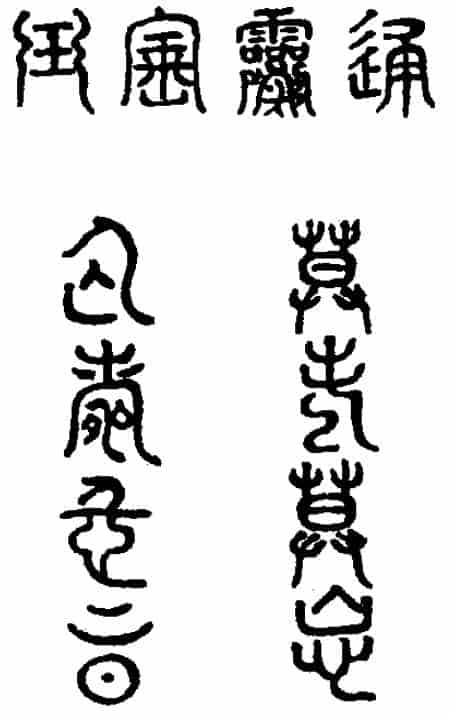
\includegraphics[width=\textwidth]{images/yu-1.JPG}
         \caption*{通灵宝玉正面图式:通灵宝玉,莫失莫忘,仙寿恒昌}
         %\label{fig:y equals x}
     \end{subfigure}
     \hfill
     \begin{subfigure}[b]{0.45\textwidth}
	     %\caption{通灵宝玉反面图式}
         \centering
         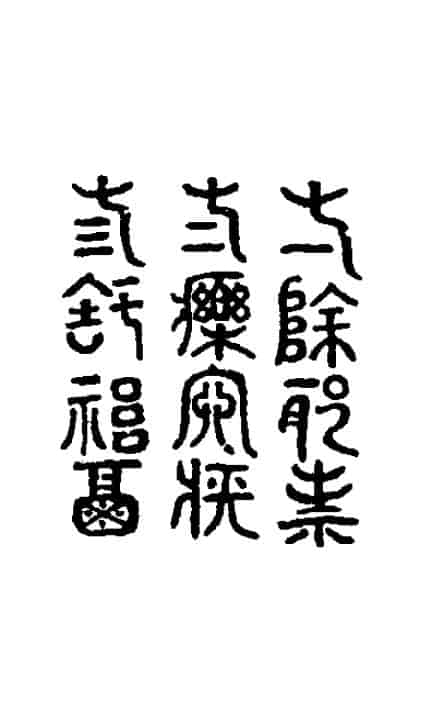
\includegraphics[width=\textwidth]{images/yu-2.JPG}
         \caption*{通灵宝玉反面图式:一除邪祟,二疗冤疾,三知祸福}%不添加*,导致输出标号(a),(b)。
         %添加*不输出编号,没有英文字符混杂         %\label{fig:three sin x}
     \end{subfigure}
        %\caption{通灵宝玉}
        %\label{fig:three graphs}
\end{figure}
宝钗看毕,\jia{余亦想见其物矣。
前回中总用草蛇灰线写法,至此方细细写出,正是大关节处。
}又从翻过正面来细看,\jia{可谓真奇之至。
}口内念道:“莫失莫忘,仙寿恒昌。
”\jia{是心中沉吟,神理。
}\jia{《石头记》立誓一笔不写一家文字。
}念了两遍,乃回头向莺儿笑道:“你不去倒茶,也在这里发呆作什么?”\jia{请诸公掩卷合目想其神理,想其坐立之势,想宝钗面上口中。
真妙!}莺儿嘻嘻笑道:“我听这两句话,倒像和姑娘的项圈上的两句话是一对儿。
”\jia{又引出一个金项圈来,莺儿口中说出方妙。
}\jia{恨颦儿不早来听此数语,若使彼闻之,不知又有何等妙论趣语以悦我等心臆。
}宝玉听了,忙笑道:“原来姐姐那项圈上也有八个字,\jia{补出素日眼中虽见而实未留心。
}
我也鉴赏鉴赏!”宝钗道:“你别听他的话,没有什么字。
”宝玉笑央:“好姐姐,你怎么瞧我的呢!”宝钗被他缠不过,因说道:“是个人给了两句吉利话儿,\zhu{“是个人”:己、庚、蒙、戚等本作“也是个人”。}\meng{“也是个”等字移换得巧妙,其雅量尊重在不言之表。
}
所以錾上了,
\zhu{錾(音“赞”):雕刻。}
叫天天带着,不然,沉甸甸的有什么趣儿。
”\jia{一句骂死天下浓妆艳饰富贵中之脂妖粉怪。
}一面说,一面解排扣,\jia{细。
}从里面大红袄上\meng{打开,好看煞人。
}将那珠宝晶莹黄金灿烂的璎珞掏将出来。
\zhu{璎珞:联缀起来的珠玉。}
\jia{按,璎珞者,颈饰也!想近俗即呼为项圈者是矣。
}宝玉忙托了锁看时,果然一面有四个篆字,两面八个,共成两句吉谶。
\zhu{
谶:音“衬”,预言。
吉谶:预示吉利的话。
}亦曾按式画下形相:\par
\clearpage
\begin{figure}[h]
     \centering
     \caption{宝钗的璎珞(金锁)}
     \begin{subfigure}[b]{0.45\textwidth}
	     %\caption{璎珞正面式}
         \centering
         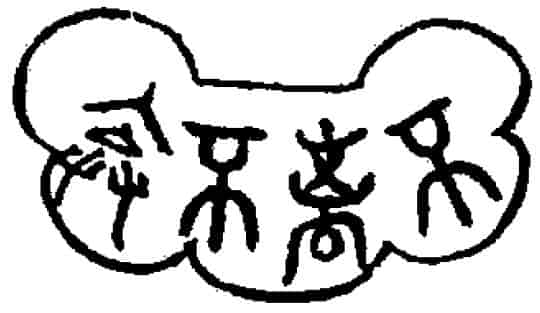
\includegraphics[width=\textwidth]{images/jin-1.JPG}
         \caption*{璎珞正面图式:不离不弃}
         %\label{fig:y equals x}
     \end{subfigure}
     \hfill
     \begin{subfigure}[b]{0.45\textwidth}
	     %\caption{璎珞反面式}
         \centering
         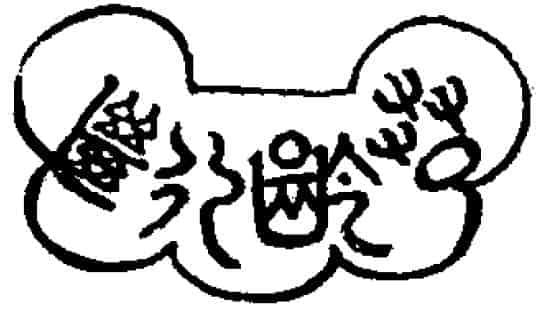
\includegraphics[width=\textwidth]{images/jin-2.JPG}
         \caption*{璎珞反面图式:芳龄永继}
         %\label{fig:three sin x}
     \end{subfigure}
        %\caption{璎珞}
        %\label{fig:three graphs}
\end{figure}
\jia{合前读之,岂非一对?}\ji{“不离不弃”与“莫失莫忘”相对,所谓愈出愈奇。
}
\jia{“芳龄永继”又与“仙寿恒昌”一对。
请合而读之。
问诸公历来小说中,可有如此可巧奇妙之文,以换新眼目?
}\par
宝玉看了,也念两遍,又念自己的两遍,因笑问:“姐姐这八个字倒真与我的是一对。
”\jia{余亦谓是一对,不知干支中四柱八字可与卿亦对否?
\zhu{
四柱八字:旧时星相家以人出生的年、月、日、时为四柱,合四柱的干支为八字,
就是人们常说的生辰八字,再把这八个字按五行生克加以推算,又称“五行八字”。
}
\ping{这个批书人看来是宝钗宝玉金玉良缘的拥趸。}
}
\jia{花看半开,酒饮微醉,此文字是也。
}莺儿笑道:“是个癞头和尚送的,他说必须錾在金器上……”\meng{和尚在幻境中作如此勾当,亦属多事。
\ping{
黛玉遇到的和尚是来救命的,宝钗遇到的和尚是来送姻缘的,
所以这条评语讽刺宝钗遇到的和尚不清心寡欲反而“作如此勾当”。
}
}宝钗不待说完,便嗔他不去倒茶,\meng{“嗔”字一截,截得妙。
}一面又问宝玉从那里来。
\jia{妙神妙理,请观者自思。
}\par
宝玉与宝钗相近,只闻一阵阵凉森森甜丝丝的幽香,\meng{这方是花香袭人正意。
}竟不知系何香气,遂问:“姐姐熏的是什么香?我竟从未闻见过这味儿。
”\jia{不知比“群芳髓”又何如?}宝钗笑道:“我最怕熏香,好好的衣服,熏的烟燎火气的。
”\jia{真真骂死一干浓妆艳饰鬼怪。
}宝玉道:“既如此,这是什么香?”宝钗想了一想,笑道:“是了,是我早起吃了丸药的香气。
”\jia{点“冷香丸”。
}宝玉笑道:“什么丸药这么好闻?好姐姐,给我一丸尝尝。
”\jia{仍是小儿语气。
究竟不知别个小儿,只宝玉如此。
}宝钗笑道:“又混闹了,一个药也是混吃的?”\par
一语未了,\meng{每善用此等转换法。
}忽听外面人说:“林姑娘来了。
”\jia{紧处愈紧,密不容针之文。
}话犹未了,林黛玉已摇摇\jia{二字画出身。
}的走了进来,一见了宝玉,便笑道:“嗳哟,我来的不巧了!”\jia{奇文,我实不知颦儿心中是何丘壑。
}\meng{怪急语。
}宝玉等忙起身笑让坐,宝钗因笑道:“这话怎么说?”\meng{不得不问。
}黛玉笑道:“早知他来,我就不来了。
”\meng{更叫人急煞。
}宝钗道:“我更不解这意。
”黛玉笑道:“要来时一群都来,要不来一个也不来,今儿他来了,明儿我再来,如此间错开了来着,岂不天天有人来了?\jia{强词夺理。
}\ping{调侃得妙,圆场得巧。
}也不至于太冷落,也不至于太热闹了。
\jia{好点缀。
}姐姐如何反不解这意思?”\jia{吾不知颦儿以何物为心为齿为口为舌,实不知胸中有何丘壑。
}\par
宝玉因见他外面罩着大红羽缎对衿褂子,\zhu{羽缎:又称羽毛缎,一种毛织品,疏细者称羽纱,厚密者称羽缎,着水不湿,可御雨雪。
衿:也作「襟」,衣服前面有钮扣开合的部分。
对衿:前幅均分为两片,中间系扣。
}\jia{岔开文字,避繁章法,妙极妙极!}\meng{又一转换。
若无此则必有宝玉之穷究,而宝钗之重复,加长无味。
此等文章是《西游记》的请观世音菩萨,菩萨一到,无不扫地完结者。
}因问:“下雪了么?”地下婆娘们道:“下了这半日雪珠儿了。
”宝玉道:“取了我的斗篷来了不曾?”黛玉便道:“是不是?我来了你就该去了。
”\jia{实不知有何丘壑。
}宝玉笑道:“我多早晚说要去了?不过是拿来预备着。
”宝玉的奶母李嬷嬷因说道:“天又下雪,也好早晚的了,就在这里同姐姐妹妹一处顽顽罢。
姨妈那里摆茶果子呢。
我叫丫头去取了斗篷来,说给小幺儿们散了罢。
”宝玉应允。
李嬷嬷出去,命小厮们都各散去不提。
\meng{极力写嬷嬷周旋,是反衬下文。
\zhu{反衬:这里李嬷嬷留宝玉在薛姨妈家,后面又因劝宝玉在薛姨妈家别饮酒而发生不愉快。}
}\par
这里薛姨妈已摆了几样细巧茶果,留他们吃茶。
\jia{是溺爱,非势利。
}
宝玉因夸前日在那府里珍大嫂子的好鹅掌、鸭信。
\zhu{鸭信:鸭舌头,可制成名菜。
信:舌头。
}\jia{为前日秦钟之事恐观者忘却,故忙中闲笔,重一渲染。
}薛姨妈听了,忙也把自己糟的取了些来与他尝。
\jia{是溺爱,非夸富。
}\meng{不写酒先写糟,将糟引酒。
}宝玉笑道:“这个须得就酒才好。
”薛姨妈便命人去灌了些上等的酒来。
\jia{愈见溺爱。
}
李嬷嬷便上来道:“姨太太,酒倒罢了。
”\jia{余最恨无调教之家,任其子侄肆行哺啜,
\zhu{
哺:音“补”,咀嚼,吃。
啜:音“辍”四声,喝;吃。
}
观此则知大家风范。
}宝玉笑央道:“好妈妈,我只吃一钟。
”李嬷嬷道:“不中用!当着老太太、太太,那怕你吃一坛呢。
想那日我眼错不见一会,不知是那一个没调教的,只图讨你的好儿,不管别人死活,给了你一口酒吃,葬送的我挨了两日骂。
姨太太不知道,他性子又可恶,\jia{补出素日。
}吃了酒更弄性。
\ping{伏“贾宝玉大醉绛芸轩”。
}有一日老太太高兴了,又尽着他吃,什么日子又不许他吃,何苦我白赔在里面。
\ping{李嬷嬷并非真为宝玉健康而劝阻宝玉饮酒,而是因为贾母和王夫人还没有同意宝玉饮酒。如果宝玉饮酒没有报备并得到批准,那么事后问责会追查到作为奶母的李嬷嬷监管照顾不周。如果宝玉饮酒得到准许,李嬷嬷是不会百般阻拦闹没趣的。}
”\jia{浪酒闲茶,原不相宜。
}
\meng{嬷嬷口气。
}\ping{李嬷嬷一席话处处从己处出发,即使有关心宝玉身体的心思也难被察觉,被厌恶真是理所当然。
}薛姨妈笑道:“老货,\jia{二字如闻。
}你只放心吃你的去。
我也不许他吃多了。
便是老太太问,有我呢。
”一面令小丫鬟:“来,让你奶奶们去,也吃杯搪搪雪气。
\zhu{搪:音“糖”,抵挡。}
”那李嬷嬷听如此说,只得和众人且去吃些酒水。
这里宝玉又说:“不必烫热了,我只爱吃冷的。
”薛姨妈忙道:“这可使不得,吃了冷酒,写字手打飐儿。
”\zhu{打飐儿:即打颤儿,发抖。
}\jia{酷肖。
}\meng{点石成金。
}宝钗笑道:“宝兄弟,亏你每日家杂学旁收的,\zhu{
家:一作“价”,语尾助词,无义。
杂学旁收:相对于应世举业的“正途”学问而言,即不去攻读《四书》《五经》时文八股而爱好诗词曲赋小说戏曲以至茶酒医药等闲杂学问。
}\jia{着眼。
若不是宝卿说出,竟不知玉卿日就何业。
}\jia{在宝卿口中说出玉兄学业,是作微露卸春挂之萌耳,是书勿看正面为幸。
\ping{这条脂评令人费解。
}\ping{宝钗对宝玉读什么书一清二楚,可见早就盯上他了。
“微露卸春挂之萌”:微:稍微。
露卸:显示。
春:可能指科举考试,即春闱。
乡试在秋天,称为“秋闱”;会试在春天,称为“春闱”。
闱(音“围”):指考场。
挂:谋求。《庄子·渔夫》:“好经大事,变更易常,以挂功名,谓之叨。”王先谦集解:“以幸功名。”
这句话可能是说宝钗日后规劝宝玉科举的苗头从现在就萌发了,这里做好铺垫,后文规劝方不突然。
}}难道就不知道酒性最热,若热吃下去,发散的就快,若冷吃下去,便凝结在内,以五脏去暖他,岂不受害?从此还不快不要吃那冷的呢。
”\jia{知命知身,识理识性,博学不杂,
\zhu{博学不杂:应该是说宝钗虽然博学多才,但是不至于因杂学而误了正业。}
庶可称为佳人。
可笑别小说中一首歪诗,几句淫曲,便自佳人相许,岂不丑杀?}宝玉听这话有情理,\jia{宝玉亦听的出有情理的话来,与前问读书家务,并皆大奇之事。
}便放下冷的,命人暖来方饮。
\par
黛玉磕着瓜子儿,只抿着嘴笑。
\jia{实不知其丘壑,自何处设想而来?}
\meng{笑的毒。
}可巧\jia{又用此二字。
}黛玉的小丫鬟雪雁走来,与黛玉送小手炉来,黛玉因含笑问他说:“谁叫你送来的?难为他费心,那里就冷死了我!”\jia{吾实不知何为心,何为齿、口、舌。
}\ping{宝钗劝宝玉不要吃冷酒,宝玉接受建议。
宝钗对宝玉影响力之大,令黛玉嫉妒。
黛玉通过“那里就冷死了我”实际上是在说:冷酒怎么就不能喝了,宝玉你怎么对宝钗她的话言听计从呢?}雪雁道:“紫鹃\jia{鹦哥改名也。
}姐姐\jia{又顺笔带出一个妙名来,洗尽春花腊梅等套。
}怕姑娘冷,使我送来的。
”黛玉一面接了,抱在怀中,笑道:“也亏你倒听他的话。
我平日和你说的,全当耳旁风,怎么他说了你就依,比圣旨还快呢!”\jia{要知尤物方如此,莫作世俗中一味酸妒狮吼辈看去。
}\meng{句句尖刺,可恨可爱,而句意毫无滞碍。
}宝玉听这话,知是黛玉借此奚落他,\ping{指桑骂槐,表面上说雪雁不听自己的话反而听紫鹃的话,实际上说宝玉不听自己的话反而听宝钗的话。
}也无回复之词,只嘻嘻的笑了两阵罢了。
\jia{这才好,这才是宝玉。
}宝钗素知黛玉是如此惯了的,也不去睬他。
\jia{浑厚天成,这才是宝钗。
}薛姨妈因道:“你素日身子弱,禁不得冷的,他们记挂着你倒不好?”\ping{薛姨妈看不懂,想要哄劝缓和局面,却不经意间给黛玉出了一道难以回答的问题,如果回答不好,很可能被人看作是不领情的冷血之人。
}黛玉笑道:“姨妈不知道。
幸亏是姨妈这里,倘或在别人家,人家岂不恼?\meng{又转出此等言语,令人疼煞黛玉,敬煞作者。
}好说就看的人家连个手炉也没有,巴巴的从家里送个来。
不说丫头们太小心过馀,还只当我素日是这等轻狂惯了呢。
”\jia{用此一解,真可拍案叫绝,足见其以兰为心,以玉为骨,以莲为舌,以冰为神。
真真绝倒天下之裙钗矣。
}薛姨妈道:“你是个多心的,有这样想。
我就没这样心。
”\par
说话时,宝玉已是三杯过去。
李嬷嬷又上来拦阻。
宝玉正在心甜意洽之时,和宝黛姊妹说说笑笑的,\jia{试问石兄:比当日青埂峰猿啼虎啸之声何如?}那肯不吃。
宝玉只得屈意央告:“好妈妈,我再吃两钟就不吃了。
”李嬷嬷道:“你可仔细老爷今儿在家,提防问你的书!”\jia{不合提此话。
这是李嬷嬷激醉了的,无怪乎后文。
一笑。
}\jia{不入耳之言是也。
}宝玉听了此话,便心中大不自在,慢慢的放下酒,垂了头。
\jia{画出小儿愁蹙之状,楔紧后文。
}黛玉先忙的说:“别扫大家的兴!舅舅\jia{二字指贾政也。
}若叫你,只说姨妈留着呢。
这个妈妈,他吃了酒,又拿我们来醒脾了!”\zhu{醒脾:即开胃;可引伸为开心。
本中医术语,是指一种治疗脾气虚寒、运化无力的方法。
}\jia{这方是阿颦真意对玉卿之文。
}一面悄推宝玉,使他赌气,一面悄悄的咕哝说:“别理那老货,咱们只管乐咱们的。
”\ping{在宝玉的饮酒问题上,宝钗黛玉争相施展自己的影响力。
}那李嬷嬷也素知黛玉的,因说道:“林姐儿,\jia{如此之称似不通,却是老妪真心道出。
}你不要助着他了。
你倒劝劝他,只怕他还听些。
”林黛玉冷笑道:“我为什么助着他?我也犯不着劝他。
你这个妈妈太小心了,往常老太太又给他酒吃,如今在姨妈这里多吃一杯,料也不妨事。
必定姨妈这里是外人,不当在这里的也未可知。
”李嬷嬷听了,又是急,又是笑,\jia{是认不得真,是不忍认真,是爱极颦儿、疼煞颦儿之意。
}说道:“真真这林姑娘,说出一句话来,比刀子还尖。
这算了什么呢。
”宝钗也忍不住笑着,把黛玉腮上一拧,\jia{我也欲拧。
}说道:“真真这个颦丫头的一张嘴,叫人恨又不是,喜欢又不是。
”\jia{可知余前批不谬。
}\meng{恨不是,喜不是,写尽一晌含容之量。
}薛姨妈一面又说:“别怕,别怕,\jia{是接前老爷问书之语。
}我的儿!来了这里没好的你吃,别把这点子东西吓的存在心里,倒叫我不安。
只管放心吃,都有我呢。
越发吃了晚饭去,便醉了,就跟着我睡罢。
”因命:“再热酒来!姨妈陪你吃两杯,可就吃饭罢。
”\jia{二语不失长上之体,且收拾若干文[字],千斤力量。
}宝玉听了,方又鼓起兴来。
\par
李嬷嬷因吩咐小丫头子们:“你们在这里小心着,我家去换了衣服就来,悄悄的回姨太太,别任他的性多给他吃。
”\meng{“家去换衣服”是含酸欲怒,“悄悄回”的光景是不露怒。
}说着便家去了。
这里虽还有三四个婆子,都是不关痛痒的,\jia{写得到。
}见李嬷嬷走了,也都悄悄的自寻方便去了。
只剩了两个小丫头子,乐得讨宝玉的欢喜。
幸而薛姨妈千哄万哄的,只容他吃了两杯,就忙收过了。
做了酸笋鸡皮汤,宝玉痛喝了两碗,吃了半碗饭碧粳粥。
\zhu{
碧粳粥:玉田碧梗米熬的粥。
玉田碧梗米在清代系贡品,清·谢墉《食味杂咏》云:“京米,近京所种统称京米,而以玉田县产者为良,粒细长,微带绿色,炊时有香。其短而大、色白不绿者,非真玉田也。”
}
\jia{美粥名。
}一时薛、林二人也吃完了饭,又酽酽的潗上茶来,\zhu{酽:音“雁”,酒、茶等味厚。
潗茶:同“沏茶”。
}每人吃了两碗。
薛姨妈方放了心。
雪雁等三四个丫头已吃了饭,进来伺候。
黛玉因问宝玉道:“你走不走?”\jia{妙问。
}\meng{“走不走”,语言真是黛玉。
}宝玉乜斜倦眼\jia{醉意。
}道:\zhu{乜(音“咩”)斜 :眯着眼睛,斜眼看人。
}“你要走,我和你一同走。
”\jia{妙答。
}\jia{此等话,阿颦心中最乐。
}\ping{谶语。
当宝玉和宝钗结婚后,宝玉“空对着、山中高士晶莹雪(薛宝钗),终不忘、世外仙姝寂寞林(林黛玉)”,最后“悬崖撒手”,“弃而为僧”。
}黛玉听说,遂起身道:“咱们来了这一日,也该回去了。
还不知那边怎么找咱们呢。
”说着,二人便告辞。
\par
小丫头忙捧过斗笠来,\jia{不漏。
}宝玉便把头略低一低,命他戴上。
那丫头便将这大红猩毡斗笠一抖,才往宝玉头上一合,宝玉便说:“罢,罢!好蠢东西,你也轻些儿!难道没见过别人\jia{“别人”者,袭人、晴雯之辈也。
}戴过的?让我自己戴罢!”黛玉站在炕沿上道:“罗唆什么,过来,我瞧瞧罢。
”宝玉忙就近前来。
黛玉用手整理,轻轻笼住束发冠,将笠沿拽在抹额之上,将那一颗核桃大的绛绒簪缨扶起,颤巍巍露于笠外。
\meng{知己最难逢,相逢意自同。
花新水上香,花下水含红。
}整理已毕,端相了端相,说道:“好了,披上斗篷罢。
”\jia{若使宝钗整理,颦卿又不知有多少文章。
}宝玉听了,方接了斗篷披上。
薛姨妈忙道:“跟你们的妈妈都还没来呢,且略等等不是。
”宝玉道:“我们倒去等他们,有丫头们跟着也够了。
”\meng{伏笔。
\ping{已有醉态的宝玉在这时就已经对奶母李嬷嬷不满了,伏下文回到绛芸轩的大闹。}
}薛姨妈不放心,便命两个妇女跟随他兄妹方罢。
他二人道了扰,一径回至贾母房中。
\par
贾母尚未用晚饭,知是薛姨妈处来,更加欢喜。
\jia{收得好极,正是写薛家母女。
}因见宝玉吃了酒,遂命他自回房去歇着,不许再出来了。
因命人好生看侍着。
忽想起跟宝玉的人来,遂问众人:“李奶子怎么不见?”\jia{细。
}\meng{逼近。
}众人不敢直说家去了,\jia{有是事,大有是事。
}
只说:“才进来的,想有事才去了。
”宝玉踉跄回头道:“他比老太太还受用呢,问他作什么!没有他只怕我还多活两日。
”一面说,一面来至自己卧室。
只见笔墨在案,\jia{如此找前文最妙,
\zhu{本回前文,众人想要宝玉写的斗方。}
且无逗榫之迹。
\zhu{
榫:音“损”,即榫头。
竹、木、石制器物或构件上利用凹凸方式相接处凸出的部分叫榫头,凹进的部分叫卯(音“毛”三声)眼。
榫在这里指文章内部联系的结构安排。
这个批语的大致意思是,赞叹文章联系结构巧妙,而且自然,没有刻意炫弄的痕迹。
}}晴雯先接出来,笑说道:“好,好,耍我!研了那些墨,早起高兴,只写了三个字,丢下笔就走了,哄的我们等了一日。
\jia{娇憨活现,余双圈不及。
\zhu{双圈:批注的方式。}
}快来给我写完这些墨才罢!”\jia{补前文之未到。
}宝玉忽然想起早起的事来,\meng{娇痴婉转,自是不凡,引后文。
}因笑道:“我写的那三个字在那里呢?”晴雯笑道:“这个人可醉了。
你头过那府里去,嘱咐我贴在这门斗上的,这会子又这么问。
\zhu{门斗:门楣,门框顶上。}
我生怕别人贴坏了,\jia{全是体贴一人。
}我亲自爬高上梯的贴上,\jia{可儿可儿。
}这会子还冻的手僵冷的呢。
” \jia{写晴雯,是晴雯走下来,断断不是袭人、平儿、莺儿等语气。
}\jia{可儿可儿。
}宝玉听了,笑\jia{是醉笑。
}道:“我忘了。
你的手冷,我替你焐着。
”\zhu{焐:覆盖裹藏某物,借以保暖或使之变暖。
}说着便伸手携了晴雯的手,同仰首看门斗上新书的三个字。
\jia{究竟不知是三个什么字,妙!}
\jia{是不作开门见山文字。
}\meng{何等景象,真是一幅教歌图。
\zhu{
教歌图:所指不明。
杜牧《寄扬州韩绰判官》:二十四桥明月夜,玉人何处教吹箫。杜牧用玩笑的口吻与韩绰调侃,问他在何处教歌妓舞女歌吹取乐,“教歌”或指此。
二十四桥:二十四座桥,或二十四美人于桥上。玉人:既可以形容美丽洁白的女子,又可比喻风流俊美的才郎,
从“教”字来看,此处玉人当指韩绰,但是二十四美人吹箫于桥上在客观上造成了“玉人”又是指月光笼罩下披着银辉的歌妓舞女的恍惚印象。
梨园位于长安宫廷禁苑梨园旁,故得名梨园。玄宗曾选坐部伎子弟三百人和宫女数百人于此学歌舞,有时亲加教正,
“教歌”或指此。后梨园泛称戏班或演戏之所。白居易《长恨歌》:梨园弟子白发新,椒房阿监青娥老。
}
}\par
一时黛玉来了,宝玉便笑道:“好妹妹,你别撒谎,你看这三个字那一个字好?”黛玉仰头看里间门斗上,新贴了三个字,写着“绛芸轩”。
\jia{出题妙。
原来是这三字。
}\meng{照应绛珠。
}黛玉笑道:“个个都好。
怎么写的这么好了?明儿也与我写一个匾。
”\jia{滑贼。
}宝玉嘻嘻的笑道:“又哄我呢。
”说着又问:“袭人姐姐呢?”\jia{断不可少。
}晴雯向里间炕上努嘴。
\jia{画。
}宝玉一看,只见袭人和衣睡着在那里。
宝玉笑道:“好,太渥早了些。
”\jia{绛芸轩中事。
}
\zhu{
渥:应为“卧”字。
另一种解释,渥:同“焐”,音“物”,用热的东西接触凉的使变暖。
宝玉睡觉前,会先让大丫鬟躺床上用身体把被窝渥热,然后自己再睡。
第五十一回,宝玉因晴雯冷,故让晴雯“进被来渥渥罢”。
针对宝玉这句话,有脂评“绛芸轩中事”。
若是普通平常的“卧”,不至于触发批书人添加评论,这也说明此处不同寻常,值得批书人感叹议论。
}
因又问晴雯道:“今儿我那府里吃早饭,有一碟子豆腐皮的包子,我想着你爱吃,和珍大奶奶说了,只说我留着晚上吃,叫人送过来的,你可吃了?”晴雯道:“快别提。
一送了来,我知道是我的,偏我才吃了饭,就搁在那里。
\meng{与颦儿抿着嘴儿笑的文字一样葫芦。
}后来李奶奶来了看见,说:‘宝玉未必吃了,拿了给我孙子吃去罢。
’他就叫人拿了家去了。
”\jia{奶母之倚势亦是常情,奶母之昏愦亦是常情。
然特于此处细写一回,与后文袭卿之酥酪遥遥一对,足见晴卿不及袭卿远矣。
\zhu{袭卿之酥酪:第十九回,李嬷嬷吃宝玉留给袭人的酥酪,袭人赶紧巧言哄住宝玉。}
余谓晴有林风,袭乃钗副,真真不错。
}\meng{嬷嬷们托大处每每如此。
\zhu{托大:骄傲自大。}
}
接着茜雪捧上茶来。
宝玉因让:“林妹妹吃茶。
”众人笑说:“林妹妹\jia{三字是接上文口气而来,非众人之称。
}\jia{醉态逼真。
}早走了,还让呢。
”\jia{写颦儿去,如此章法从何设想?奇笔奇文。
}\ping{无端令人伤感,林妹妹真走时,是不是也是如此光景,梦幻一般悄无声息去了,宝玉混沌一片,只心里还念着要给她茶吃。
}\par
宝玉吃了半碗茶,忽又想起早起的茶来,\jia{偏是醉人搜寻得出细事,亦是真情。
}因问茜雪道:“早起潗了一碗枫露茶,\jia{与“千红一窟”遥映。
}
我说过,那茶是三四次后才出色的,这会子怎么又潗了这个来?”\jia{所谓闲茶是也,与前浪酒一般起落。
}茜雪道:“我原是留着的,那会子李奶奶来了,他要尝尝,就给他吃了。
”\jia{又是李嬷,事有凑巧,如此类是。
}
宝玉听了,将手中的茶杯只顺手\jia{是醉后,故用二字,非有心动气也。
}往地下一掷,\jia{按警幻情榜,宝玉系“情不情”。
凡世间之无知无识,彼俱有一痴情去体贴。
今加“大醉”二字于石兄,是因问包子、问茶、顺手掷杯、问茜雪、撵李嬷,乃一部中未有第二次事也。
袭人数语,无言而止,石兄真大醉也。
}\jia{余亦云实实大醉也。
难辞醉闹,非薛蟠纨绔辈可比!}豁啷一声,
\zhu{豁音“或”,啷音“浪“一声。豁啷:象声词。}
打个齑粉,
\zhu{齑:音“机”。齑粉:碎成粉屑。}
泼了茜雪一裙子的茶。
又跳起来问着茜雪道:“他是你那一门子的奶奶,你们这么孝敬他?不过是仗着我小时候吃过他几日奶罢了。
\jia{真醉了。
}如今逞的他比祖宗还大了。
如今我又吃不着奶了,白白的养着祖宗作什么!撵了出去,大家干净!”\jia{真真大醉了。
}说着立刻便要去回贾母,撵他乳母。
\par
原来袭人实未睡着,不过故意装睡,引宝玉来怄他顽耍。
\zhu{怄:音“沤”,这里是撩拨逗弄、厮缠、磨人的意思。
}\meng{“只许郎看不近郎”,真是妙法。
}\ping{顽什么啊,莫非又要干那警幻所训之事?}先闻得说字、问包子等事,也还可不必起来,后来摔了茶钟,动了气,遂连忙起来解释劝阻。
早有贾母遣人来问是怎么了。
\jia{断不可少之文。
}袭人忙道:“我才倒茶来,被雪滑倒了,\jia{现成之至,瞧他写袭卿为人。
}\meng{袭人另有一段居心,一番行止。
}失了手砸了钟子。
”一面又安慰宝玉道:“你立意要撵他也好,\jia{二字奇,使人一惊。
}我们也都愿意出去,\meng{先主取西川,方得立基业,而偏不肯取,大与此意同。
\zhu{
引用三国的典故,西川刘璋听信张松、法正之言,迎接刘备入益州,想藉刘备之力,抵抗张鲁、曹操。
不料此举乃引狼入室,刘备不久借故攻击刘璋,并最终占据益州奠定蜀汉基业。
刘备在入川之初念及和刘璋的宗室关系及自己的仁义之名,没有直接采取行动。
这条评语的意思是,袭人为了劝宝玉息怒,以退为进,把宝玉的命令扩大化极端化,让宝玉自己觉得命令不切实际而放弃。
}
}不如趁势连我们一齐撵了,我们也好,你也不愁再有好的来伏侍你。
”宝玉听了这话,方无了言语,被袭人等扶至炕上,脱换了衣服。
不知宝玉口内还说些什么,只觉口齿缠绵,眼眉愈加饧涩,\zhu{
饧:音“行”,眼睛半睁半闭或呆滞无神。
饧涩:形容眼睛半睁半闭,眼光黏滞。
}\jia{二字带出平素形象。
}
忙伏侍他睡下。
袭人伸手从他项上摘下那通灵玉来,用自己的手帕包好,塞在褥下,次日戴时便冰不着脖子。
\jia{试问石兄:此一渥,
\zhu{渥:同“焐”,音“物”,用热的东西接触凉的使变暖。}
比青埂峰下松风明月如何?}那宝玉就枕便睡着了。
彼时李嬷嬷等已进来了,听见醉了,不敢前来再加触犯,只悄悄的打听睡了,方放心散去。
\jia{交代清楚。
“塞玉”一段,又为“误窃”一回伏线。
晴雯茜雪二婢又为后文先作一引。
\zhu{
“误窃”一回,前 80 回中未见,或为 80 回以后之佚稿。
第二十三回,宝玉从贾政处回来,“刚至穿堂门下”,庚辰本、有正本夹批:“妙,这便是凤姐扫雪拾玉之处。”
第十七至十八回写元春点戏,在《仙缘》戏目下,庚辰、己卯、有正本夹批:“《邯郸梦》中,伏甄宝玉送玉。”
这两条脂批所述内容,亦当为 80 回以后之佚稿。误窃、拾玉、送玉,都指宝玉所佩之通灵宝玉。
}
}\jia{偷度金针法,最巧。
\zhu{
偷度金针:
度:授与,传授。比喻把高超的技艺偷偷传授给别人。
后也以刺绣譬喻作诗文者别有巧妙,明清小说、戏剧评点家也常用来评点小说、戏剧中的巧妙章法和构思。
从《红楼梦》有关回的正文看,作批者是指曹雪芹表面在写一回事,而实际有更深的、另外的含义,或者是运用巧妙的艺术手法而不露痕迹。
}
}\par
次日醒来,\jia{以上已完正题,以下是后文引子,前文之馀波。
此回收法与前数回不同矣。
}就有人回:“那边小蓉大爷带了秦相公来拜。
”宝玉忙接了出去,领了拜见贾母。
贾母见秦钟形容标致,举止温柔,堪陪宝玉读书,\jia{娇养如此,溺爱如此。
}心中十分欢喜,便留茶留饭,又命人带去见王夫人等。
众人因素爱秦氏,今见了秦钟是这般人品,也都欢喜,临去时都有表礼。
\zhu{表礼:旧日赠送或赏赐的礼物。}
贾母又与了一个荷包并一个金魁星,\zhu{荷包:用以装药品、香料等细小物品的扁圆形绣花小袋。
金魁星:黄金铸成的魁星神像,有祝颂功名顺利的意思。
魁星:本作奎星,北斗第一星,汉代纬书《孝经援神契》有“奎主文章”之说,后遂以此星为掌文运之神。
}\jia{作者今尚记金魁星之事乎?抚今思昔,肠断心摧。
}取“文星和合”之意。
\zhu{文星和合:“文星”又称文昌星、文曲星,星相家以其为吉星、主文运、保功名。
“和合”与荷包谐音,且为中国民间所奉喜庆吉祥之神。
}\meng{雅致。
}又嘱咐他道:“你家住的远,一时寒热饥饱不便,只管住在我这里,不必限定了。
只和你宝叔在一处,别跟着那起不长进的东西学。
”\jia{总伏后文。
\zhu{下回大闹学堂。}
}秦钟一一答应,回去禀知他父亲秦业。
\jia{妙名。
业者,孽也,盖云情因孽而生也。
}\par
这秦业现任营缮郎,\zhu{营缮郎:官名。
明清时工部有营缮司,设郎中、员外郎等职。
}\jia{官职更妙,设云因情孽而缮此一书之意。
}年近七十,夫人早亡。
因当年无儿女,便向养生堂抱了一个儿子并一个女儿。
\zhu{养生堂:又叫育婴堂。
一种收养弃婴的慈善机构。
}
谁知儿子又死了,\jia{一顿。
}只剩女儿,小名唤可儿,\jia{出名。
秦氏究竟不知系出何氏,所谓寓褒贬、别善恶是也。
秉刀斧之笔、具菩萨之心亦甚难矣。
}\jia{如此写出可儿来历亦甚苦矣。
又知作者是欲天下人共来哭此情字。
}\jia{写可儿出身自养生堂,是褒中贬。
后死封龙禁尉,是贬中褒。
灵巧一至于此。
}长大时,生得形容袅娜,性格风流。
\jia{四字便有隐意。
《春秋》字法。
\zhu{
《春秋》字法:
《春秋》是孔子根据鲁史撰修的编年体史书。
古代学者说它“以一字为褒贬”,含有“微言大义”。
后来就把文笔深隐曲折、意含褒贬叫“春秋笔法”。
}
}因素与贾家有些瓜葛,故结了亲,许与贾蓉为妻。
\zhu{
贾蓉乃贾家嫡长孙,为何娶一个出身不明的女子?刘心武在《秦可卿出身未必寒微》一文中,有如下阐述:\hang
旧时无儿女,最普遍的是过继一个侄儿,秦业有这个条件,由第十六回“秦鲸卿夭逝黄泉路”宝玉跑到秦家去奔丧,
看到“两个远房婶母并几个弟兄”可知。而秦业却抱养一儿一女,最后儿子还死了,只剩女儿,令人疑窦丛生。\hang
秦可卿有贵妇大家气派,没有出身带来的自卑,甚至贾母认为秦可卿是“重孙媳中第一个得意之人”,这和秦可卿养生堂弃婴出身相矛盾。\hang
对秦可卿卧室华丽奢侈陈设的描写,用武则天、赵飞燕、杨太真、寿昌公主、同昌公主这些意象,不仅暗示秦可卿的风流,可能还在暗示秦可卿出身的高贵。\hang
可卿是太虚幻境中警幻仙姑的妹妹(第五回:吾妹一人,乳名兼美字可卿者),此可卿可能暗示彼可卿同样出身不俗。\hang
秦可卿临死托梦,嘱咐凤姐“趁今日富贵,将祖莹附近多置田庄房舍地亩”,其最重要的根据是“便是有了罪,凡物可入官,这祭祀产业连官也不入的”,迥然一个获罪被抄的富贵之家的后人的反思。\hang
秦可卿丧事隆重铺张,北静王亲来探丧上祭设路奠,而在贾敬丧事却不见北静王。秦可卿的棺木用的是义忠亲王老千岁的,非常人可享。\hang
从脂砚斋批语“秦可卿淫丧天香楼……因命芹溪删去”可见,对于秦可卿原始结局,曹雪芹进行了删节,其中可能删去了关于秦可卿真实身份的揭秘,又不能丝毫不交代她的来历,于是便到第八回末尾加了一段从养生堂抱来之类的看似明确却更含糊的文字,实际是打了一个“补丁”。 
}
那秦业五旬之上方得了秦钟。
因去岁业师亡故,未暇延请高明之士,只暂在家温习旧课。
正思要和亲家\jia{指贾珍。
}去商议,送往他家塾中,暂且不致荒废,可巧遇见了宝玉这个机会。
又知贾家塾中现今司塾的是贾代儒,\jia{随笔命名,省事。
}乃当今之老儒,秦钟此去,学业料必进益,成名可望,因此十分欢喜。
只是宦囊羞涩,\zhu{宦囊羞涩:意谓做官者手头拮据。
语本“阮囊羞涩”,见《韵府群玉·阳韵》:“阮孚持一皂囊(皂:黑),游会稽。
客问:‘囊中何物?’曰:‘但有一钱看囊,恐其羞涩’。
”}那贾府上上下下都是一双富贵眼睛,\jia{为天下读书人一哭、寒素人一哭。
}容易拿不出来,\zhu{不容易拿出来。
}又恐误了儿子的终身大事,\jia{原来读书是终身大事。
}
说不得东拼西凑的恭恭敬敬\jia{四字可思,近之鄙薄师傅者来看。
}封了二十四两贽见礼,\zhu{
贽:音“至”,古人初次拜见尊长时拿的礼物。
贽见礼:旧时学生拜见老师时所送的礼,封套上要写“贽敬”。
}\jia{可知“宦囊羞涩”与“东拼西凑”等样,是特为近日守钱虏而不使子弟读书之辈一大哭。
}\meng{父母之恩,昊天罔极。
\zhu{罔:音“网”,通「无」,没有。昊天罔极:苍天广阔无穷尽。比喻父母恩德如苍天广大,无以回报。}
}亲自带了秦钟,来代儒家拜见了。
然后听宝玉上学之日,好一同入塾。
\jia{不想浪酒闲茶一段金玉旖旎之文后,忽用此等寒瘦古拙之词收住,亦行文之大变体处。
《石头记》多用此法,历观后文便知。
}正是:\par
早知日后闲争气,岂肯今朝错读书。
\jia{这是隐语微词,岂独指此一事哉?}\jia{余则谓读书正为争气。
但此“争气”与彼“争气”不同。
写来一笑。
}\par
\qi{总评:一是先天衔来之玉,一是后天造就之金。
\zhu{宝玉宝钗金玉良缘是刻意造作,而宝玉黛玉木石前盟是天作之合。}
金玉相合,是成万物之象。
再遇水而过寒,虽有酒浆,岂能助火?因生出黛玉之讽刺,李嬷嬷之唠叨,晴雯、茜雪之嗔恼。
故不得不收功静息,涵养性天,以待再举。
识丹道者,当解吾意。
\zhu{这条评语为了用金(木)水火(土)五行解释小说情节,显得过于牵强附会。}
}
\dai{015}{宝玉宝钗互看通灵宝玉和金锁}
\dai{016}{宝玉黛玉薛姨妈家吃饭,丫鬟送手炉}
\sun{p8-1}{宝玉凤姐回家称赞秦钟,宝玉遇见门下清客}{图右侧:宝玉回到家中, 便回明贾母要约秦钟上家塾之事,这样自己有了伴读的朋友,也好发奋。
凤姐也在一旁帮着说:“改日秦钟还来拜见老祖宗呢。
”说得贾母喜欢起来。
图左侧:宝玉想起去看宝钗,谁知到了穿堂,向东北绕过厅后,遇到了门下清客詹光、单聘仁,唠叨了一会儿才走开。
}
\sun{p8-2}{贾宝玉奇缘识金锁,薛宝钗巧合认通灵,林黛玉来访梨香院}{图右侧:宝玉来到宝钗房内,问过安后,宝钗要宝玉落草时衔下来的那块玉细看。
宝钗将玉托在掌上,只见那玉大如雀卵,灿若明霞,莹润如酥,五色花纹缠护,更可怪的是,石上还镌刻着“莫失莫忘,仙寿恒昌”八字。
宝钗正轻轻念着,莺儿笑道,“我听这两句话,倒像和姑娘项圈上的两句话是一对儿。
”宝玉听了也争着要看,宝钗被缠不过,便解下来给宝玉看。
只见金锁上分明錾了“不离不弃,芳龄永继”八字,正与宝玉的那八个字是一对儿。
图左侧:说话间,黛玉走了进来。
}
\sun{p8-3}{宝玉黛玉告别同返}{黛玉因问宝玉道:“你走不走?”宝玉乜斜倦眼道:“你要走,我和你一同走。
”黛玉听说,遂起身道:“咱们来了这一日,也该回去了。
还不知那边怎么找咱们呢。
”说着,二人便告辞。
两人一起离开梨香院。
}
\sun{p8-4}{宝黛共赏绛芸轩匾,宝玉领秦钟拜贾母}{图右侧:宝玉回到房中, 想起早晨写的字,便问晴雯,晴雯说已经贴在门斗儿上了。
一时,黛玉来了, 宝玉问她哪个字写得好,黛玉仰头见是“绛芸轩”三字,说道: “个个都好。
“宝玉问:“袭人呢?”晴雯向里间炕上努嘴儿。
图左侧:次日,贾蓉带了秦钟来,宝玉领了去拜见贾母。
贾母见秦钟形容标致,举止温柔,堪陪宝玉读书,心中十分喜欢。
}